\makeatletter \def\NR@nopatch@beamer{} \makeatother %Temporary due to bug on 17 May

\documentclass{beamer}\usepackage[]{graphicx}\usepackage[]{xcolor}
% maxwidth is the original width if it is less than linewidth
% otherwise use linewidth (to make sure the graphics do not exceed the margin)
\makeatletter
\def\maxwidth{ %
  \ifdim\Gin@nat@width>\linewidth
    \linewidth
  \else
    \Gin@nat@width
  \fi
}
\makeatother

\definecolor{fgcolor}{rgb}{0.345, 0.345, 0.345}
\newcommand{\hlnum}[1]{\textcolor[rgb]{0.686,0.059,0.569}{#1}}%
\newcommand{\hlstr}[1]{\textcolor[rgb]{0.192,0.494,0.8}{#1}}%
\newcommand{\hlcom}[1]{\textcolor[rgb]{0.678,0.584,0.686}{\textit{#1}}}%
\newcommand{\hlopt}[1]{\textcolor[rgb]{0,0,0}{#1}}%
\newcommand{\hlstd}[1]{\textcolor[rgb]{0.345,0.345,0.345}{#1}}%
\newcommand{\hlkwa}[1]{\textcolor[rgb]{0.161,0.373,0.58}{\textbf{#1}}}%
\newcommand{\hlkwb}[1]{\textcolor[rgb]{0.69,0.353,0.396}{#1}}%
\newcommand{\hlkwc}[1]{\textcolor[rgb]{0.333,0.667,0.333}{#1}}%
\newcommand{\hlkwd}[1]{\textcolor[rgb]{0.737,0.353,0.396}{\textbf{#1}}}%
\let\hlipl\hlkwb

\usepackage{framed}
\makeatletter
\newenvironment{kframe}{%
 \def\at@end@of@kframe{}%
 \ifinner\ifhmode%
  \def\at@end@of@kframe{\end{minipage}}%
  \begin{minipage}{\columnwidth}%
 \fi\fi%
 \def\FrameCommand##1{\hskip\@totalleftmargin \hskip-\fboxsep
 \colorbox{shadecolor}{##1}\hskip-\fboxsep
     % There is no \\@totalrightmargin, so:
     \hskip-\linewidth \hskip-\@totalleftmargin \hskip\columnwidth}%
 \MakeFramed {\advance\hsize-\width
   \@totalleftmargin\z@ \linewidth\hsize
   \@setminipage}}%
 {\par\unskip\endMakeFramed%
 \at@end@of@kframe}
\makeatother

\definecolor{shadecolor}{rgb}{.97, .97, .97}
\definecolor{messagecolor}{rgb}{0, 0, 0}
\definecolor{warningcolor}{rgb}{1, 0, 1}
\definecolor{errorcolor}{rgb}{1, 0, 0}
\newenvironment{knitrout}{}{} % an empty environment to be redefined in TeX

\usepackage{alltt}
\usepackage{graphicx}
\usepackage{verbatim}
\usepackage{etoolbox}
\usepackage{everysel}
% \usepackage{enumitem}

%% This package allows text highlighting
\usepackage{soul}

%% This sets the theme of the presentation which controls
%% the formatting of the slides
\usetheme{Boadilla}

%% Turn off the navigation symbols
\setbeamertemplate{navigation symbols}{} 

%% Change the default itemize [ball]s to [circle]s
\setbeamertemplate{itemize items}[circle]

%% Change the default enumerate [ball]s to plain text
\setbeamertemplate{enumerate items}[default]

%% Load the enumitem package and ensure it works nicely with beamer
% \setitemize{label=\usebeamerfont*{itemize item}
%   \usebeamercolor[fg]{itemize item}
%   \usebeamertemplate{itemize item}}
% \setenumerate{label=\usebeamerfont*{enumerate item}
%   \usebeamercolor[fg]{enumerate item}
%   \usebeamertemplate{enumerate item}}

%% Set the author block so STATS 201/8 appears on every
\author{STATS 201/8}

%% Clear the date block
\date{}


\setbeamercolor{title}{bg=blue!40}
\setbeamerfont{title}{size=\LARGE,series=\bfseries}

%%Sectioning commands
\setbeamercolor{section title}{bg=blue!20}
\setbeamerfont{section title}{size=\large}

\setbeamertemplate{section page}{%
    \begingroup
        \begin{beamercolorbox}[sep=10pt,center,rounded=true,shadow=true]{section title}
        \usebeamerfont{section title}Section~\thechapter.\thesection \newline \insertsection\par
        \end{beamercolorbox}
		\vfill
    \endgroup
}

\newcommand{\BeginSection}[1]{\section{#1} \frame{\sectionpage}}
%\AtBeginSection[]{%
%    \begin{frame}
%        \sectionpage
%    \end{frame}
%}


%% This makes all equations blue
\AtBeginEnvironment{equation*}{\color{blue}}
\AtBeginEnvironment{align*}{\color{blue}}
\everymath{\color{blue}}

%% This puts a 0 point space between paragraphs, means we don't need to use vspace, or list environments if 
%% we don't want to
\setlength{\parskip}{0pt}


%% Russell: removes spaces after R input/output?
\setlength{\topsep}{0.5mm}

%% David: In addition to Russel's command to remove spaces after R input/output, these commands remove the space between R input/output.
%% Stackoverflow link: https://stackoverflow.com/questions/35734525/reduce-space-between-code-chunks-and-code-output-in-rmarkdown-beamer-presentatio
%% \setlength{\OuterFrameSep}{-2pt}
\makeatletter
\preto{\@verbatim}{\topsep=-1pt \partopsep=-1pt }
\makeatother

%% Some useful colors
\definecolor{darkgreen}{rgb}{0.176,0.486,0.031}
\definecolor{redbrown}{HTML}{950605}
\definecolor{darkred}{HTML}{d80605}


%% nice little macro for changing the font of R code
\newcommand{\rcode}[1]{\protect{\color{darkgreen}\texttt{#1}}}

%% macro for bold blue italics
\newcommand{\blueBoldEmph}[1]{{\color{blue}\textbf{\emph{#1}}}}

% ~iid macro
\newcommand{\iid }{\stackrel{iid}{\sim}}

%% Macro for t-test amd P-value
\newcommand{\ttest}{\emph{t}-test}
\newcommand{\pval}{\emph{P}-value}

%% Statistics operators 
\DeclareMathOperator{\Bias}{Bias}
\DeclareMathOperator{\Cov}{Cov}
\DeclareMathOperator*{\Cor}{Cor}
\DeclareMathOperator{\E}{E}
\DeclareMathOperator{\MSE}{MSE}
\DeclareMathOperator{\Odds}{Odds}
\DeclareMathOperator{\OR}{OR}
\DeclareMathOperator{\PMSE}{PMSE}
\DeclareMathOperator{\sd}{sd}
\DeclareMathOperator{\se}{se}
\DeclareMathOperator*{\Var}{Var}
\DeclareMathOperator{\logit}{logit}

%% Should see if can make this a mathop
\newcommand{\comb}[2]{\mbox{$\big(_{#2}^{#1}\big)$}}




% \setlength{\parskip}{7pt}
% \setlength{\topsep}{0mm} %To reduce line spacing in R output
\IfFileExists{upquote.sty}{\usepackage{upquote}}{}
\begin{document}
\newcommand{\thechapter}{14}

\title{Chapter \thechapter: \\ Poisson modelling of count data: \newline Two examples.}
\institute{University of Auckland}




\begin{frame}
\titlepage
\end{frame}



\begin{frame}[t]
\frametitle{Learning Outcomes}
In this chapter you will learn about using a Poisson regression GLM to model:
\begin{center}
\vspace{16pt}
\begin{minipage}{0.9\textwidth}
  \begin{itemize}
    \item Earthquake frequencies using earthquake magnitude (numeric) and location (factor) as explanatory variables.
    \item Snapper counts using location (factor) and reservation status (factor) as explanatory variables.
  \end{itemize}
\end{minipage}
\end{center}

\end{frame}


%%%%%%%%%%%%%%%%%%%%%%%%%%%%%%%%%%%%%%%%%%%%%%%%%%%%%%%%%%%%%%%%%%%%%%%%%%%%%%%%%%%%%%%%%%%
\BeginSection{Example 1: Earthquake frequency}
%%%%%%%%%%%%%%%%%%%%%%%%%%%%%%%%%%%%%%%%%%%%%%%%%%%%%%%%%%%%%%%%%%%%%%%%%%%%%%%%%%%%%%%%%%%



\begin{frame}
\frametitle{Earthquake magnitudes}
\framesubtitle{The Gutenberg-Richter law}

The Gutenberg-Richter law says that the expected number of earthquakes in a given period of time
decreases multiplicatively with their magnitude.
The formula is
\[ \log_{10} N = a - b M \]
where $N$ is the expected number of earthquakes of magnitude $M$ or more
on the Richter scale. 
Here, $a$ and $b$ are unknown parameters.

\medskip
The Richter scale is logarithmic (base 10). 
So, for example, an earthquake that registers 5.0 on the Richter scale has a shaking amplitude 10 times that of an earthquake that registers 4.0. It can be shown that this corresponds to 30 times the release of energy.

\medskip
FYI, the most powerful earthquake ever recorded was in Chile in 1960, measuring 9.5 on the
Richter scale.
The largest known seismic events on earth have been caused by asteroid impact,
exceeding 13 on the Richter scale.
\end{frame}


\begin{frame}
\frametitle{Earthquake magnitudes\ldots}
\framesubtitle{The Gutenberg-Richter law\ldots}

After applying a healthy dash of calculus,
this formula can be re-expressed in a form that is more familiar to us
\[ E[Y|x] = \exp(\beta_0 + \beta_1 x) \]
where $Y$ is the number of earthquakes having magnitude between
$x-\delta$ and $x+\delta$.\footnote{
In the above formula, $\beta_0$ and $\beta_1$ depend on $a$, $b$ and $\delta$
in a complicated way that we are not going to concern ourselves with.}

\medskip

E.g., if $x=6$ and $\delta=0.125$ then $Y$ is the number of earthquakes
between 5.875 and 6.125 in magnitude.

\medskip

The above formula should look familiar. It is the one we use for a Poisson regression GLM when there is a single numeric explanatory variable $x$.
\end{frame}




\begin{frame}[fragile]
\frametitle{Sthn California and Washington earthquakes, 1987--2019}
The research question is to quantify the rate of decrease in earthquake
frequency (with increasing magnitude) in both Southern California (SC) and the State of Washington (WA),
and to assess whether these rates are the same.

\begin{knitrout}\scriptsize
\definecolor{shadecolor}{rgb}{0.969, 0.969, 0.969}\color{fgcolor}\begin{kframe}
\begin{alltt}
\hlstd{> }\hlstd{Quakes.df}\hlkwb{=}\hlkwd{read.table}\hlstd{(}\hlstr{"Data/EarthquakeMagnitudes.txt"}\hlstd{,}\hlkwc{header}\hlstd{=}\hlnum{TRUE}\hlstd{)}
\hlstd{> }\hlstd{Quakes.df}\hlopt{$}\hlstd{Locn}\hlkwb{=}\hlkwd{as.factor}\hlstd{(Quakes.df}\hlopt{$}\hlstd{Locn)}
\hlstd{> }\hlkwd{subset}\hlstd{(Quakes.df,}\hlkwc{subset}\hlstd{=}\hlkwd{c}\hlstd{(Locn}\hlopt{==}\hlstr{"SC"}\hlstd{))[}\hlnum{1}\hlopt{:}\hlnum{4}\hlstd{,]} \hlcom{#Print first 4 SC observations}
\end{alltt}
\begin{verbatim}
  Locn Magnitude Freq
1   SC      5.25   32
2   SC      5.50   27
3   SC      5.75   10
4   SC      6.00    9
\end{verbatim}
\begin{alltt}
\hlstd{> }\hlkwd{subset}\hlstd{(Quakes.df,}\hlkwc{subset}\hlstd{=}\hlkwd{c}\hlstd{(Locn}\hlopt{==}\hlstr{"WA"}\hlstd{))[}\hlnum{1}\hlopt{:}\hlnum{4}\hlstd{,]} \hlcom{#Print first 4 WA observations}
\end{alltt}
\begin{verbatim}
   Locn Magnitude Freq
10   WA      5.25   13
11   WA      5.50    6
12   WA      5.75    2
13   WA      6.00    1
\end{verbatim}
\end{kframe}
\end{knitrout}
Here we have one explanatory variable that is a factor variable,
and another that is numeric. 
We have seen this before in Chapter 8, and we handle it in much the same way as before,
but using \rcode{glm} instead of \rcode{lm}.

\end{frame}


\begin{frame}[fragile]
\frametitle{Sthn CA and WA earthquakes, 1987--2019\ldots}
\framesubtitle{Plotting the data}
\begin{knitrout}\scriptsize
\definecolor{shadecolor}{rgb}{0.969, 0.969, 0.969}\color{fgcolor}\begin{kframe}
\begin{alltt}
\hlstd{> }\hlkwd{plot}\hlstd{(Freq}\hlopt{~}\hlstd{Magnitude,}\hlkwc{data}\hlstd{=Quakes.df,}\hlkwc{pch}\hlstd{=}\hlkwd{substr}\hlstd{(Locn,}\hlnum{1}\hlstd{,}\hlnum{1}\hlstd{))}
\end{alltt}
\end{kframe}
\end{knitrout}



\begin{figure}
  \centering
  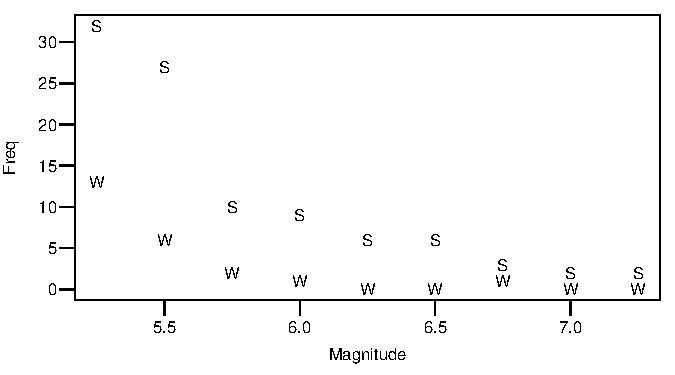
\includegraphics[scale=0.8]{figure/RC-H14-003}
\end{figure}

The data look consistent with an exponential decay. It is not clear if the rates of exponential decay are the same.
\end{frame}



\begin{frame}[fragile]
\frametitle{Sthn CA and WA earthquakes, 1987--2019\ldots}
\framesubtitle{Model fit and assumption checking}
Recall from Chapter 8 that we fit the interaction model first, and then simplify if possible.

\begin{knitrout}\scriptsize
\definecolor{shadecolor}{rgb}{0.969, 0.969, 0.969}\color{fgcolor}\begin{kframe}
\begin{alltt}
\hlstd{> }\hlstd{Quake.gfit} \hlkwb{=} \hlkwd{glm}\hlstd{(Freq} \hlopt{~} \hlstd{Locn} \hlopt{*} \hlstd{Magnitude,} \hlkwc{family} \hlstd{= poisson,}
\hlstd{+ }                 \hlkwc{data} \hlstd{= Quakes.df)}
\hlstd{> }\hlkwd{plot}\hlstd{(Quake.gfit,} \hlkwc{which} \hlstd{=} \hlnum{1}\hlstd{)}
\end{alltt}
\end{kframe}
\end{knitrout}



\begin{figure}
  \centering
  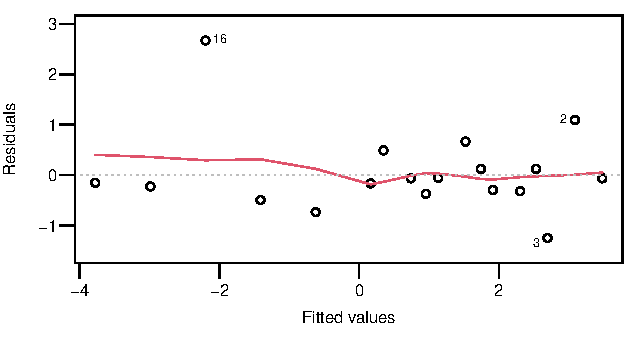
\includegraphics[scale=0.7]{figure/RC-H14-007}
\end{figure}

Looks OK, notwithstanding that observation 16 has a high residual. This observation has low expected value (approx $\exp(-2)$), so this residual is not reliable and no cause for concern. 
\end{frame}



\begin{frame}[fragile]
\frametitle{Sthn CA and WA earthquakes, 1987--2019\ldots}
\framesubtitle{Checking influence}

\begin{knitrout}\scriptsize
\definecolor{shadecolor}{rgb}{0.969, 0.969, 0.969}\color{fgcolor}\begin{kframe}
\begin{alltt}
\hlstd{> }\hlkwd{plot}\hlstd{(Quake.gfit,} \hlkwc{which} \hlstd{=} \hlnum{4}\hlstd{)}
\end{alltt}
\end{kframe}
\end{knitrout}



\begin{figure}
  \centering
  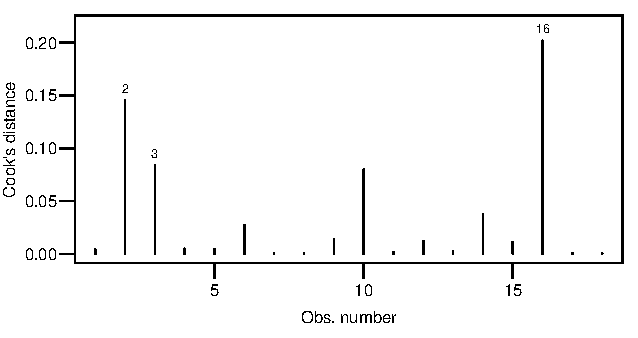
\includegraphics[scale=0.7]{figure/RC-H14-007b}
\end{figure}

No influential points. 
\end{frame}



\begin{frame}[fragile]
\frametitle{Sthn CA and WA earthquakes, 1987--2019\ldots}
\framesubtitle{Summary output}
\begin{knitrout}\scriptsize
\definecolor{shadecolor}{rgb}{0.969, 0.969, 0.969}\color{fgcolor}\begin{kframe}
\begin{alltt}
\hlstd{> }\hlkwd{summary}\hlstd{(Quake.gfit)}
\end{alltt}
\end{kframe}
\end{knitrout}

\begin{knitrout}\scriptsize
\definecolor{shadecolor}{rgb}{0.969, 0.969, 0.969}\color{fgcolor}\begin{kframe}
\begin{verbatim}
Call:
glm(formula = Freq ~ Locn * Magnitude, family = poisson, data = Quakes.df)

Coefficients:
                 Estimate Std. Error z value Pr(>|z|)    
(Intercept)       11.6923     1.1762   9.941  < 2e-16 ***
LocnWA             7.3923     3.9500   1.871   0.0613 .  
Magnitude         -1.5648     0.2055  -7.616 2.61e-14 ***
LocnWA:Magnitude  -1.5884     0.7199  -2.206   0.0274 *  
---
(Dispersion parameter for poisson family taken to be 1)

    Null deviance: 176.1767  on 17  degrees of freedom
Residual deviance:   8.2295  on 14  degrees of freedom
\end{verbatim}
\end{kframe}
\end{knitrout}

\medskip

The residual deviance of 8.23 is less than the 14 residual degrees of freedom, so there won't be any problems with the variance check.   

\begin{knitrout}\scriptsize
\definecolor{shadecolor}{rgb}{0.969, 0.969, 0.969}\color{fgcolor}\begin{kframe}
\begin{alltt}
\hlstd{> }\hlnum{1} \hlopt{-} \hlkwd{pchisq}\hlstd{(}\hlnum{8.23}\hlstd{,} \hlnum{14}\hlstd{)}
\end{alltt}
\begin{verbatim}
[1] 0.8770025
\end{verbatim}
\end{kframe}
\end{knitrout}
\end{frame}


\begin{frame}[fragile]
\frametitle{Sthn CA and WA earthquakes, 1987--2019\ldots}

The interaction term \pval{} is 0.027, so we conclude that the effect of magnitude is different at the two locations.
\bigskip

Next, lets quantify these rates. First, for Southern California:
\begin{knitrout}\scriptsize
\definecolor{shadecolor}{rgb}{0.969, 0.969, 0.969}\color{fgcolor}\begin{kframe}
\begin{alltt}
\hlstd{> }\hlstd{Quake.cis} \hlkwb{=} \hlkwd{confint}\hlstd{(Quake.gfit)}
\end{alltt}


{\ttfamily\noindent\itshape\color{messagecolor}{Waiting for profiling to be done...}}\begin{alltt}
\hlstd{> }\hlkwd{exp}\hlstd{(Quake.cis[}\hlnum{3}\hlstd{,])}
\end{alltt}
\begin{verbatim}
    2.5 %    97.5 % 
0.1374743 0.3082437 
\end{verbatim}
\begin{alltt}
\hlstd{> }\hlcom{## To interpret as percentage decreases}
\hlstd{> }\hlnum{100}\hlopt{*}\hlstd{(}\hlnum{1}\hlopt{-}\hlkwd{exp}\hlstd{(Quake.cis[}\hlnum{3}\hlstd{,]))}
\end{alltt}
\begin{verbatim}
   2.5 %   97.5 % 
86.25257 69.17563 
\end{verbatim}
\end{kframe}
\end{knitrout}
\end{frame}



\begin{frame}[fragile]
\frametitle{Sthn CA and WA earthquakes, 1987--2019\ldots}
We change the baseline to get the rate for Washington:

\begin{knitrout}\scriptsize
\definecolor{shadecolor}{rgb}{0.969, 0.969, 0.969}\color{fgcolor}\begin{kframe}
\begin{alltt}
\hlstd{> }\hlstd{Quakes.df}\hlopt{$}\hlstd{Locn2}\hlkwb{=}\hlkwd{factor}\hlstd{(Quakes.df}\hlopt{$}\hlstd{Locn,}\hlkwc{levels}\hlstd{=}\hlkwd{c}\hlstd{(}\hlstr{"WA"}\hlstd{,}\hlstr{"SC"}\hlstd{))}
\hlstd{> }
\hlstd{> }\hlstd{Quake2.gfit}\hlkwb{=}\hlkwd{glm}\hlstd{(Freq}\hlopt{~}\hlstd{Locn2}\hlopt{*}\hlstd{Magnitude,}\hlkwc{family}\hlstd{=poisson,}\hlkwc{data}\hlstd{=Quakes.df)}
\hlstd{> }\hlstd{(Quake.WA.ci} \hlkwb{=} \hlkwd{exp}\hlstd{(}\hlkwd{confint}\hlstd{(Quake2.gfit)[}\hlnum{3}\hlstd{,]))}
\end{alltt}


{\ttfamily\noindent\itshape\color{messagecolor}{Waiting for profiling to be done...}}\begin{verbatim}
      2.5 %      97.5 % 
0.009077661 0.140175445 
\end{verbatim}
\begin{alltt}
\hlstd{> }\hlcom{## To interpret as percentage decreases}
\hlstd{> }\hlnum{100}\hlopt{*}\hlstd{(}\hlnum{1} \hlopt{-} \hlstd{Quake.WA.ci)}
\end{alltt}
\begin{verbatim}
   2.5 %   97.5 % 
99.09223 85.98246 
\end{verbatim}
\end{kframe}
\end{knitrout}
\end{frame}



\begin{frame}[fragile]
\frametitle{Sthn CA and WA earthquakes, 1987--2019\ldots}
\framesubtitle{Executive Summary}
Our Executive Summary would say that the rate of decline in the frequency of
earthquakes (with increasing magnitude) is more rapid in WA than CA.
\bigskip

In WA, there is a 86 to 99\% drop in the expected number of earthquakes for a one
unit increase in their magnitude on the Richter scale. 
In CA, the decrease is between 69 to 86\%.
\end{frame}



%%%%%%%%%%%%%%%%%%%%%%%%%%%%%%%%%%%%%%%%%%%%%%%%%%%%%%%%%%%%%%%%%%%%%%%%%%%%%%%%%%%%%%%%%%%
\BeginSection{Example 2: Snapper counts in and around marine reserves}
%%%%%%%%%%%%%%%%%%%%%%%%%%%%%%%%%%%%%%%%%%%%%%%%%%%%%%%%%%%%%%%%%%%%%%%%%%%%%%%%%%%%%%%%%%%



\begin{frame}[fragile]
\frametitle{Snapper counts in and around marine reserves}
Baited underwater video (BUV) is an established tool for counting fish such as snapper.
\medskip

BUV was used at two coastal locations in New Zealand, Leigh and Hahei. 
Each location has a marine reserve. 
The BUV was deployed at sites inside the marine reserve, 
and at sites just outside the reserve.
There was a total of 18 sites.
\medskip

The three variables measured were
\begin{itemize}
\item Count of snapper
\item Location (Leigh or Hahei)
\item Reservation status (Yes or No)
\end{itemize}
\medskip

It was of interest to explore the count of snapper with regard
to location and reservation status.
\end{frame}


\begin{frame}[fragile]
\frametitle{Snapper counts in and around marine reserves\ldots}

\begin{knitrout}\scriptsize
\definecolor{shadecolor}{rgb}{0.969, 0.969, 0.969}\color{fgcolor}\begin{kframe}
\begin{alltt}
\hlstd{> }\hlstd{Snap.df}\hlkwb{=}\hlkwd{read.table}\hlstd{(}\hlstr{"Data/SnapperCROPvsHAHEI.txt"}\hlstd{,}\hlkwc{header}\hlstd{=}\hlnum{TRUE}\hlstd{)}
\hlstd{> }\hlkwd{with}\hlstd{(Snap.df,\{Locn}\hlkwb{=}\hlkwd{as.factor}\hlstd{(Locn); Reserve}\hlkwb{=}\hlkwd{as.factor}\hlstd{(Reserve)\})}
\hlstd{> }\hlstd{Snap.df}
\end{alltt}
\begin{verbatim}
    Locn Reserve Freq
1  Leigh       N    2
2  Leigh       N    1
3  Leigh       N    0
4  Leigh       Y    5
5  Leigh       Y   11
6  Leigh       Y    7
7  Leigh       Y    8
8  Leigh       Y    7
9  Leigh       Y   14
10 Hahei       N    1
11 Hahei       N    0
12 Hahei       N    1
13 Hahei       N    0
14 Hahei       Y    3
15 Hahei       Y    2
16 Hahei       Y    1
17 Hahei       Y    5
18 Hahei       Y    3
\end{verbatim}
\end{kframe}
\end{knitrout}
\end{frame}


\begin{frame}[fragile]
\frametitle{Snapper counts in and around marine reserves\ldots}
\framesubtitle{Plotting the data}

\begin{knitrout}\scriptsize
\definecolor{shadecolor}{rgb}{0.969, 0.969, 0.969}\color{fgcolor}\begin{kframe}
\begin{alltt}
\hlstd{> }\hlkwd{interactionPlots}\hlstd{(Freq} \hlopt{~} \hlstd{Locn} \hlopt{+} \hlstd{Reserve,} \hlkwc{data} \hlstd{= Snap.df)}
\end{alltt}
\end{kframe}
\end{knitrout}

\begin{knitrout}\scriptsize
\definecolor{shadecolor}{rgb}{0.969, 0.969, 0.969}\color{fgcolor}
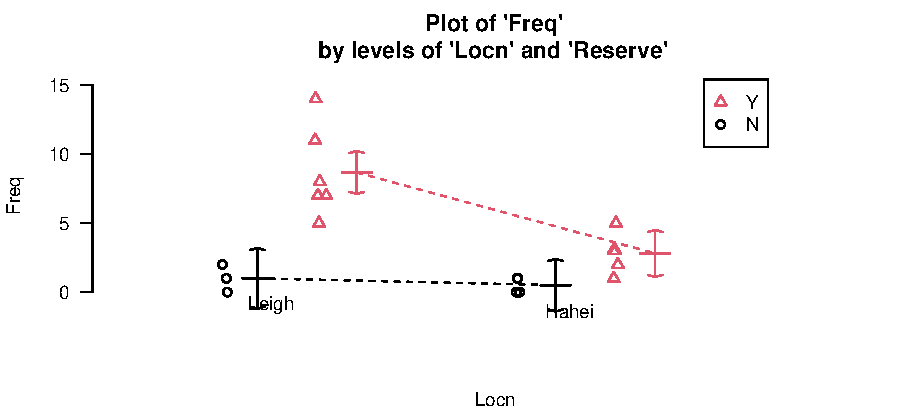
\includegraphics[width=\maxwidth]{figure/RC-H14-015-1} 
\end{knitrout}

{\bf NOTE:} Parallel lines no longer corresponds to lack of interaction.
{\bf Why?}
\end{frame}


\begin{frame}[fragile]
\frametitle{Snapper counts in and around marine reserves\ldots}
\framesubtitle{Model fit and assumption checking}
There are two categorical explanatory variables, so we follow the steps from Chapter 12. First, we fit an interaction model:
\medskip

\begin{knitrout}\scriptsize
\definecolor{shadecolor}{rgb}{0.969, 0.969, 0.969}\color{fgcolor}\begin{kframe}
\begin{alltt}
\hlstd{> }\hlstd{Snap.glm} \hlkwb{=} \hlkwd{glm}\hlstd{(Freq} \hlopt{~} \hlstd{Locn}\hlopt{*}\hlstd{Reserve,} \hlkwc{family} \hlstd{= poisson,} \hlkwc{data} \hlstd{= Snap.df)}
\hlstd{> }\hlkwd{plot}\hlstd{(Snap.glm,} \hlkwc{which} \hlstd{=} \hlnum{1}\hlstd{)}
\end{alltt}
\end{kframe}
\end{knitrout}



\begin{figure}
  \centering
  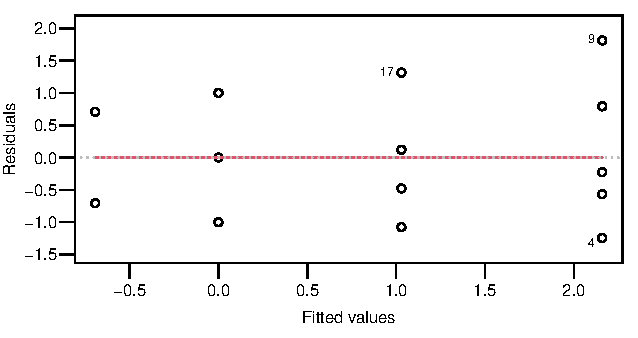
\includegraphics[scale=0.7]{figure/RC-H14-017}
\end{figure}

Looks fine.
\end{frame}


\begin{frame}[fragile]
\frametitle{Snapper counts in and around marine reserves\ldots}
\framesubtitle{Influence checking}

\begin{knitrout}\scriptsize
\definecolor{shadecolor}{rgb}{0.969, 0.969, 0.969}\color{fgcolor}\begin{kframe}
\begin{alltt}
\hlstd{> }\hlkwd{plot}\hlstd{(Snap.glm,} \hlkwc{which} \hlstd{=} \hlnum{4}\hlstd{)}
\end{alltt}
\end{kframe}
\end{knitrout}



\begin{figure}
  \centering
  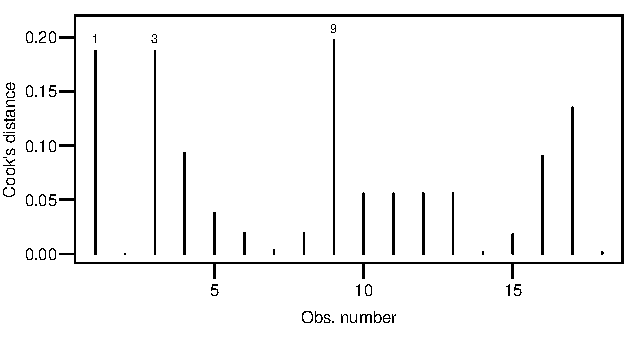
\includegraphics[scale=0.9]{figure/RC-H14-017b}
\end{figure}

No overly influential points.
\end{frame}


\begin{frame}[fragile]
\frametitle{Snapper counts in and around marine reserves\ldots}
\framesubtitle{Assumption checking\ldots}

\begin{knitrout}\scriptsize
\definecolor{shadecolor}{rgb}{0.969, 0.969, 0.969}\color{fgcolor}\begin{kframe}
\begin{alltt}
\hlstd{> }\hlkwd{summary}\hlstd{(Snap.glm)}
\end{alltt}
\end{kframe}
\end{knitrout}

\begin{knitrout}\scriptsize
\definecolor{shadecolor}{rgb}{0.969, 0.969, 0.969}\color{fgcolor}\begin{kframe}
\begin{verbatim}
Call:
glm(formula = Freq ~ Locn * Reserve, family = poisson, data = Snap.df)

Coefficients:
                   Estimate Std. Error z value Pr(>|z|)  
(Intercept)         -0.6931     0.7071  -0.980   0.3270  
LocnLeigh            0.6931     0.9129   0.759   0.4477  
ReserveY             1.7228     0.7559   2.279   0.0227 *
LocnLeigh:ReserveY   0.4367     0.9612   0.454   0.6496  
---
(Dispersion parameter for poisson family taken to be 1)

    Null deviance: 70.453  on 17  degrees of freedom
Residual deviance: 14.678  on 14  degrees of freedom
\end{verbatim}
\end{kframe}
\end{knitrout}

\medskip

The residual deviance is 14.678 on 14 dof. No problems there.

\begin{knitrout}\scriptsize
\definecolor{shadecolor}{rgb}{0.969, 0.969, 0.969}\color{fgcolor}\begin{kframe}
\begin{alltt}
\hlstd{> }\hlnum{1} \hlopt{-} \hlkwd{pchisq}\hlstd{(}\hlnum{14.678}\hlstd{,} \hlnum{14}\hlstd{)}
\end{alltt}
\begin{verbatim}
[1] 0.4005141
\end{verbatim}
\end{kframe}
\end{knitrout}

\end{frame}


\begin{frame}[fragile]
\frametitle{Snapper counts in and around marine reserves\ldots}
\framesubtitle{Apply Occam's razor}
We see that the interaction between Location and Reserve is not required,
so lets redo the \rcode{glm} without the interaction.
\medskip

\begin{knitrout}\scriptsize
\definecolor{shadecolor}{rgb}{0.969, 0.969, 0.969}\color{fgcolor}\begin{kframe}
\begin{alltt}
\hlstd{> }\hlstd{Snap2.glm} \hlkwb{=} \hlkwd{glm}\hlstd{(Freq} \hlopt{~} \hlstd{Locn} \hlopt{+} \hlstd{Reserve,} \hlkwc{family} \hlstd{= poisson,} \hlkwc{data} \hlstd{= Snap.df)}
\hlstd{> }\hlkwd{summary}\hlstd{(Snap2.glm)}
\end{alltt}
\end{kframe}
\end{knitrout}

\begin{knitrout}\scriptsize
\definecolor{shadecolor}{rgb}{0.969, 0.969, 0.969}\color{fgcolor}\begin{kframe}
\begin{verbatim}
Call:
glm(formula = Freq ~ Locn + Reserve, family = poisson, data = Snap.df)

Coefficients:
            Estimate Std. Error z value Pr(>|z|)    
(Intercept)  -0.9491     0.4884  -1.943 0.051990 .  
LocnLeigh     1.0894     0.2845   3.829 0.000128 ***
ReserveY      2.0105     0.4646   4.328 1.51e-05 ***
---
(Dispersion parameter for poisson family taken to be 1)

    Null deviance: 70.453  on 17  degrees of freedom
Residual deviance: 14.879  on 15  degrees of freedom
\end{verbatim}
\end{kframe}
\end{knitrout}

\end{frame}

\begin{frame}[fragile]
\frametitle{Snapper counts in and around marine reserves\ldots}
The residual deviance still indicates no evidence of a problem:
\begin{knitrout}\scriptsize
\definecolor{shadecolor}{rgb}{0.969, 0.969, 0.969}\color{fgcolor}\begin{kframe}
\begin{alltt}
\hlstd{> }\hlnum{1} \hlopt{-} \hlkwd{pchisq}\hlstd{(}\hlnum{14.879}\hlstd{,} \hlnum{15}\hlstd{)}
\end{alltt}
\begin{verbatim}
[1] 0.4601677
\end{verbatim}
\end{kframe}
\end{knitrout}
\bigskip

Lets calculate some confidence intervals, 
remembering to exponentiate them to get the multiplicative effects of
location and reservation status.

\begin{knitrout}\scriptsize
\definecolor{shadecolor}{rgb}{0.969, 0.969, 0.969}\color{fgcolor}\begin{kframe}
\begin{alltt}
\hlstd{> }\hlstd{(Snap.cis} \hlkwb{<-} \hlkwd{exp}\hlstd{(}\hlkwd{confint}\hlstd{(Snap2.glm)))}
\end{alltt}


{\ttfamily\noindent\itshape\color{messagecolor}{Waiting for profiling to be done...}}\begin{verbatim}
                2.5 %     97.5 %
(Intercept) 0.1298697  0.9105143
LocnLeigh   1.7443515  5.3626745
ReserveY    3.3224830 21.3481546
\end{verbatim}
\end{kframe}
\end{knitrout}

\end{frame}

\begin{frame}[fragile]
\frametitle{Snapper counts in and around marine reserves\ldots}
\framesubtitle{Executive Summary}
We conclude that the expected count of snapper is between 3.3 and 21.3 times as high in marine reserves than in the area just outside of the reserve.
\bigskip

Moreover, the Leigh location has higher expected snapper counts than Hahei,
 - they are between 1.7 and 5.4 times as high at Leigh.
\end{frame}


\begin{frame}[fragile]
\frametitle{Closing remark -- use of \rcode{anova} with a GLM}
In situations where we need to test a joint hypothesis (see Chapter 9) we can continue to use the \rcode{anova} function.
\medskip

However, be aware that \rcode{anova} for GLMs can use several different methods for calculating the appproximate \pval{} for the joint hypothesis. We recommend using \rcode{test="Chisq"}. 
\medskip

By way of example:"
\begin{knitrout}\scriptsize
\definecolor{shadecolor}{rgb}{0.969, 0.969, 0.969}\color{fgcolor}\begin{kframe}
\begin{alltt}
\hlstd{> }\hlstd{Snap.anova}\hlkwb{=}\hlkwd{anova}\hlstd{(Snap2.glm,}\hlkwc{test}\hlstd{=}\hlstr{"Chisq"}\hlstd{)}
\hlstd{> }\hlkwd{data.frame}\hlstd{(Snap.anova)} \hlcom{#Using data.frame removes extraneous output}
\end{alltt}
\begin{verbatim}
        Df Deviance Resid..Df Resid..Dev     Pr..Chi.
NULL    NA       NA        17   70.45338           NA
Locn     1 22.65585        16   47.79753 1.937697e-06
Reserve  1 32.91888        15   14.87866 9.608571e-09
\end{verbatim}
\end{kframe}
\end{knitrout}

Note that the \pval{} for the reserve effect is different from that obtained from \rcode{summary(Snap2.glm)}, but both \pval{s} tell the same story -- a very highly significant effect of reserve.
\end{frame}

\end{document}
